\subsection{The Isomorphism Theorems}

Let $G$ be a group.

\begin{exercise}[3.3.1]
    Let $F$ be a finite field of order $q$ and let $n \in \zp$.
	Prove that $|\gl_N(F) : \splin_n(F)| = q - 1$. [See \exref{3.1.35}.]
\end{exercise}

\begin{sol}
    In \exref{3.1.35}, we showed that $\splin_n(F) \nsub \gl_n(F)$ and that $\gl_n(F)/\splin_n(F) \cong F\unt$.
	Since $F$ is a finite field of order $q$, then $\abs{F\unt} = q - 1$.
	We then have that $|\gl_n(F) : \splin_n(F)| = \abs{F\unt} = q - 1$.
\end{sol}

\begin{spex}[3.3.2]
    Prove all parts of the Lattice Isomorphism Theorem.
\end{spex}

\begin{sol}
    Let $\acal = \set{A \leq G \mid N \subseteq A}$ be the set of subgroups of $G$ containing $N$.
	Let $\bar{\acal} = \set{\bar A \leq \bar G}$ be the set of subgroups of $\bar G = G/N$.
	Define the map
    \[
    	\phi : \acal \to \bar{\acal} \quad \text{by} \quad \phi(A) = \bar A = A/N
    \]
    We first show that $\phi(A) \leq \bar G$.
	Since $1 \in A$ for any $A \in \acal$, then $1N = N \in \bar A$ so that $\bar 1 \in \bar A$, hence $\bar A$ is nonempty.
	Let $\bar a, \bar b \in \bar A$, where $a, b \in A$.
	Since $A \leq G$, then $ab\inv \in A$, hence
    \[
    	\bar a \bar b\inv = \bar{ab\inv} \in \bar A
    \]
    so that $\bar A \leq \bar G$.

    Next, we show that $\phi$ is surjective.
	Let $\bar A \in \bar{\acal}$, and let $\pi : G \to \bar G$ be the natural projection homomorphism.
	Consider $\pi\inv(\bar A)$.
	Since $\pi$ is a homomorphism, then $\pi\inv(\bar A) \leq G$.
	Moreover, since $\bar 1 \in \bar A$, then $N = \pi\inv(\bar 1) \subseteq \pi\inv(\bar A)$ so that $\pi\inv(\bar A) \in \acal$.
	Note that
    \[
    	\phi(\pi\inv(\bar A)) = \pi\inv(\bar A)/N = \bar A
    \]
    so that $\phi$ is surjective.
	To show that $\phi$ is injective, suppose $\phi(A) = \phi(B)$ for some $A, B \in \acal$.
	Then $\bar A = \bar B$ implies that for some $a \in A$, there is some $b \in B$ such that $\bar a = \bar b$, hence $aN = bN$ so that $b\inv a \in N \subseteq B$.
	It follows that $a = b(b\inv a) \in B$, hence $A \subseteq B$.
	A similar argument shows that $B \subseteq A$, hence $A = B$ so that $\phi$ is injective.
	Therefore, $\phi$ is a bijection.
    \begin{enumerate}
        \item 
        \begin{itemize}
            \item[\rightimp] Suppose $A \leq B$ for $A, B \in \acal$.
	Let $\bar a \in \bar A$ for some $a \in A$.
	Since $A \leq B$, then $a \in B$ so that $\bar a \in \bar B$, hence $\bar A \leq \bar B$.
            \item[\leftimp] Suppose $\bar A \leq \bar B$ for $A, B \in \acal$.
	Let $a \in A$ for some $a \in A$.
	Then $\bar a \in \bar A$ so that $\bar a \in \bar B$, hence there is some $b \in B$ such that $\bar a = \bar b$.
	It follows that $aN = bN$ so that $b\inv a \in N \subseteq B$, hence $a = b(b\inv a) \in B$.
	Therefore, $A \leq B$.
        \end{itemize}
        \item Define the map
        \[
        	\psi : B/A \to \bar B / \bar A \quad \text{by} \quad \psi(bA) = \bar b \bar A
        \]
        for $b \in B$.
	To show $\psi$ is well-defined, suppose $b_1A = b_2A$ for some $b_1, b_2 \in B$.
	Then $b_2\inv b_1 \in A$, hence $\bar{b_2\inv b_1} \in \bar A$.
	Then $\bar{b_1} bar A = \bar{b_2} \bar A$, hence $\psi(b_1A) = \psi(b_2A)$.

        Suppose $bA \in \ker\psi$.
	Then $\psi(bA) = \bar A$ so that $\bar b \bar A = \bar A$.
	Then $\bar b \in \bar A$, hence $bN \in A/N$, and $b \in A$.
	Then $bA = A$ which is the identity in $B/A$ so that $\ker\psi = 1$, hence $\psi$ is injective.
	To show that $\psi$ is surjective, let $\bar b \bar A \in \bar B/\bar A$ for $\bar b \in B$.
	By definition of $\bar B$, there exists $b \in B$ such that $\bar b = bN$.
	Then $\psi(bA) = \bar b \bar A$, hence $\psi$ is surjective.
	Lastly, for any $b_1A, b_2A \in B/A$,
        \[
        	\psi(b_1A \cdot b_2A) = \psi(b_1b_2A) = \bar{b_1b_2} \bar A = \bar b_1 \bar b_2 \bar A = \psi(b_1A) \cdot \psi(b_2A)
        \]
        so that $\psi$ is a homomorphism.
	Therefore, $\psi$ is an isomorphism and $|B : A| = |B/A| = |\bar B / \bar A| = |\bar B : \bar A|$.
        \item Let $\bar x \in \bar{\gen{A, B}}$.
	Then $x \in \gen{A, B}$ so that $x = x_1x_2 \ldots x_n$ where $x_i \in A \cup B$ for each $1 \leq i \leq n$.
	It follows that
        \[
        	\bar x = \bar{x_1x_2} \ldots \bar{x_n}
        \]
        where $\bar{x_i} \in \bar A \cup \bar B$ for each $1 \leq i \leq n$, hence $\bar x \in \gen{\bar A, \bar B}$, and $\bar{\gen{A, B}} \subseteq \gen{\bar A, \bar B}$. 
        
        Conversely, let $\bar x \in \gen{\bar A, \bar B}$.
	Then $\bar x = \bar{x_1x_2} \ldots \bar{x_n}$ where $\bar{x_i} \in \bar A \cup \bar B$ for each $1 \leq i \leq n$.
	It follows that $x = x_1x_2 \ldots x_n$ where $x_i \in A \cup B$ for each $1 \leq i \leq n$, hence $x \in \gen{A, B}$ so that $\bar x \in \bar{\gen{A, B}}$.
	Therefore, $\bar{\gen{A, B}} = \gen{\bar A, \bar B}$.
        \item Let $\bar x \in \bar{A \cap B}$.
	Then $x \in A \cap B$ so that $x \in A$ and $x \in B$, hence $\bar x \in \bar A$ and $\bar x \in \bar B$, so that $\bar x \in \bar A \cap \bar B$.
	It follows that $\bar{A \cap B} \subseteq \bar A \cap \bar B$.
        
        Conversely, let $\bar x \in \bar A \cap \bar B$.
	Then $\bar x \in \bar A$ and $\bar x \in \bar B$, so that $x \in A$ and $x \in B$, hence $x \in A \cap B$ so that $\bar x \in \bar{A \cap B}$.
	Therefore, $\bar{A \cap B} = \bar A \cap \bar B$.
        \item 
        \begin{itemize}
            \item[\rightimp] Suppose $A \nsub G$ for some $A \in \acal$.
	Let $\bar g \in \bar G$ and $\bar a \in \bar A$ for some $g \in G$ and $a \in A$.
	Note that
            \[
            	(\bar g)(\bar a)(\bar g)\inv = \bar{gag\inv}
            \]
            Since $A \nsub G$, then $gag\inv \in A$, hence $\bar{gag\inv} \in \bar A$.
	It follows that $(\bar g)(\bar a)(\bar g)\inv \in \bar A$, hence $\bar A \nsub \bar G$.
            \item[\leftimp] Suppose $\bar A \nsub \bar G$ for some $A \in \acal$.
	Let $g \in G$ and $a \in A$.
	Since $\bar{gag\inv} = (\bar g)(\bar a)(\bar g)\inv \in \bar A$, then $gag\inv N \in A/N$, hence $gag\inv \in A$.
	It follows that $A \nsub G$. \qh
        \end{itemize}
    \end{enumerate}
\end{sol}

\begin{exercise}[3.3.3]
    Prove that if $H$ is a normal subgroup of $G$ of prime index $p$ then for all $K \leq G$ either
    \begin{enumerate}
        \item[(i)] $K \leq H$ or
        \item[(ii)] $G = HK$ and $|K : K \cap H| = p$.
    \end{enumerate}
\end{exercise}

\begin{sol}
    Since $H \nsub G$ and $K \leq G$, then $HK \leq G$ by Corollary 3.15.
	By Proposition 3.14, $HK = KH$.
	By \exref{3.2.11}, we have
    \[
    	|G : H| = |G : HK| \cdot |HK : H|
    \]
    Since $|G : H| = p$, we have two cases:
    \begin{enumerate}
        \item If $|G : HK| = 1$, then $G = HK = KH$.
	By the Second Isomorphism Theorem, we have
        \[
        	K/(K \cap H) \cong KH/H = G/H
        \]
        so that $|K : K \cap H| = |KH : H| = |G : H| = p$.
        \item If $|G : HK| = p$, then $|HK : H| = 1$, hence $HK = H$.
	It follows that $K \leq H$. \qh
    \end{enumerate}
\end{sol}

\begin{exercise}[3.3.4]
    Let $C$ be a normal subgroup of the group $A$ and let $D$ be a normal subgroup of the group $B$.
	Prove that $(C \times D) \nsub (A \times B)$ and $(A \times B)/(C \times D) \cong (A/C) \times (B/D)$.
\end{exercise}

\begin{sol}
    Define the map
    \[
    	\phi : A \times B \to (A/C) \times (B/D) \quad \text{by} \quad \phi(a, b) = (aC, bD)
    \]
    for $a \in A$ and $b \in B$.
	It is easy to see that $\phi$ is well-defined.
	Moreover, for any $(a_1, b_1), (a_2, b_2) \in A \times B$,
    \[
    	\phi((a_1, b_1)(a_2, b_2)) = \phi(a_1a_2, b_1b_2) = (a_1a_2C, b_1b_2D) = (a_1C, b_1D)(a_2C, b_2D) = \phi(a_1, b_1) \phi(a_2, b_2)
    \]
    so that $\phi$ is a homomorphism.
	To show that $\phi$ is surjective, let $(aC, bD) \in (A/C) \times (B/D)$ for some $a \in A$ and $b \in B$.
	Then $\phi(a, b) = (aC, bD)$, hence $\phi$ is surjective.
	Lastly, suppose $(a, b) \in \ker\phi$.
	Then $\phi(a, b) = (C, D)$ so that $aC = C$ and $bD = D$.
	It follows that $a \in C$ and $b \in D$, hence $(a, b) \in C \times D$.
	Therefore, $\ker\phi = C \times D$, so that by the First Isomorphism Theorem, $C \times D \nsub A \times B$ and
    \[
    	(A \times B)/(C \times D) \cong (A/C) \times (B/D). \qh
    \]
\end{sol}

\begin{exercise}[3.3.5]
    Let $QD_{16} = \gen{\sigma, \tau}$ be the quasidihedral group of order 16 in \exref{2.5.11}.
	Prove that $\gen{\sigma^4}$ is normal in $QD_{16}$ and use the Lattice Isomorphism Theorem to draw the lattice of subgroups of $QD_{16}/\gen{\sigma^4}$.
	Which group of order 8 has the same lattice as this quotient?
	Use generators and relations for $QD_{16}$ to decide the isomorphism type of this group.
\end{exercise}

\begin{sol}
    Note that $\tau\sigma^4\tau = \tau\tau\sigma^{12} = \sigma^4$, hence $\gen{\sigma^4} \nsub QD_{16}$.
	By the Lattice Isomorphism Theorem, we may draw the following diagram:
    \begin{center}
        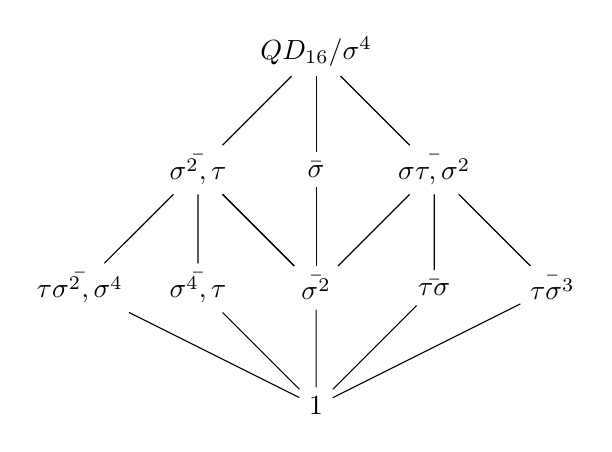
\begin{tikzpicture}[scale=1.5]
            \node (d8) at (0, 0) {$QD_{16}/\gen{\sigma^4}$};
            
            \node (sr2) at (-1, -1) {$\bar{\gen{\sigma^2, \tau}}$};
            \node (r) at (0, -1) {$\bar{\gen\sigma}$};
            \node (rsr2) at (1, -1) {${\bar{\gen{\sigma\tau, \sigma^2}}}$};

            \node (s) at (-2, -2) {$\bar{\gen{\tau\sigma^2, \sigma^4}}$};
            \node (r2s) at (-1, -2) {$\bar{\gen{\sigma^4, \tau}}$};
            \node (r2) at (0, -2) {$\bar{\gen{\sigma^2}}$};
            \node (rs) at (1, -2) {$\bar{\gen{\tau\sigma}}$};
            \node (r3s) at (2, -2) {$\bar{\gen{\tau\sigma^3}}$};
            
            \node (1) at (0, -3) {1};

            \draw (1) -- (s) -- (sr2) -- (d8);
            \draw (1) -- (r2s) -- (sr2);
            \draw (1) -- (r2) -- (sr2);
            \draw (1) -- (rs) -- (rsr2) -- (d8);
            \draw (1) -- (r3s) -- (rsr2);
            \draw (r2) -- (r) -- (d8);
            \draw (r2) -- (sr2);
            \draw (r2) -- (rsr2);
        \end{tikzpicture}
    \end{center}
    Moreover, $\bar{\sigma^4} = \bar{\tau^2} = \bar 1$ and $\bar{\tau\sigma} = \bar{\sigma^3\tau} = \bar{\sigma\inv\tau}$, then the generators $\bar\sigma$ and $\bar\tau$ satisfy the relations as $r$ and $s$ do in $D_8$, hence $QD_{16}/\gen{\sigma^4} \cong D_8$.
\end{sol}

\begin{exercise}[3.3.6]
    Let $M = \gen{u, v}$ be the modular group of order 16 in \exref{2.5.14}.
	Prove that $\gen{v^4}$ is normal in $M$ and use the Lattice Isomorphism Theorem to draw the lattice of subgroups of $M/\gen{v^4}$.
	Which group of order 8 has the same lattice as this quotient?
	Use generators and relations for $M$ to decide the isomorphism type of this group.
\end{exercise}

\begin{sol}
    Note that $uv^4u = uuv^{20} = v^4$, hence $\gen{v^4} \nsub M$.
	By the Lattice Isomorphism Theorem, we may draw the following diagram:
    \begin{center}
        \begin{tikzpicture}[every node/.style=on grid]
            \node (G) {$M/\gen{v^4}$};

            \node (y) [below left=of G] {$\bar{\gen v}$};
            \node (xy) [below=of G] {$\bar{\gen{uv}}$};
            \node (x y2) [below right=of G] {$\bar{\gen{u, v^2}}$};

            \node (y2) [below right=of y] {$\bar{\gen{v^2}}$};
            \node (xy2) [below=of x y2] {$\bar{\gen{uv^2}}$};
            \node (x y4) [below right=of x y2] {$\bar{\gen{u, v^4}}$};

            \node (y4) [below right=of y2] {$\bar{\gen{v^4}}$};

            \draw (y4) -- (y2) -- (y) -- (G);
            \draw (y4) -- (x y4) -- (x y2) -- (G);
            \draw (y4) -- (xy2) -- (x y2);
            \draw (y2) -- (xy) -- (G);
            \draw (y2) -- (x y2);
        \end{tikzpicture}
    \end{center}
    Moreover, $\bar{v^4} = \bar{u^2} = \bar 1$ and $\bar{vu} = \bar{uv^5} = \bar{uv}$ so that the generators of $M/\gen{v^4}$ satisfy the relations as $a$ and $b$ do in $Z_2 \times Z_4$, whose presentation is given in \exref{2.5.12}.
	Then $M/\gen{v^4} \cong Z_2 \times Z_4$.
\end{sol}

\begin{exercise}[3.3.7]
    Let $M$ and $N$ be normal subgroups of $G$ such that $G = MN$.
	Prove that $G/(M \cap N) \cong (G/M) \times (G/N)$. [Draw the lattice.]
\end{exercise}

\begin{sol}
    The lattice is given as the following, where double lines represent the quotient group $G/(M \cap N)$:
    \begin{center}
        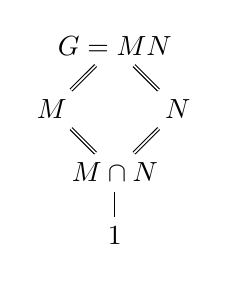
\begin{tikzpicture}[scale=0.8]
            \node (MN) at (0, 0) {$G = MN$};
            \node (M) at (-1, -1) {$M$};
            \node (N) at (1, -1) {$N$};
            \node (MnN) at (0, -2) {$M \cap N$};
            \node (1) at (0, -3) {1};

            \draw (1) -- (MnN);
            \draw [double] (MnN) -- (M) -- (MN);
            \draw [double] (MnN) -- (N) -- (MN);
        \end{tikzpicture}
    \end{center}
    Consider the mapping
    \[
    	\phi : G \to (G/M) \times (G/N) \quad \text{by} \quad \phi(g) = (gM, gN)
    \]
    for $g \in G$.
	It is easy to see that $\phi$ is well-defined.
	Moreover, for any $g_1, g_2 \in G$,
    \[
    	\phi(g_1g_2) = (g_1g_2M, g_1g_2N) = (g_1M, g_1N)(g_2M, g_2N) = \phi(g_1)\phi(g_2)
    \]
    so that $\phi$ is a homomorphism.
	To show that $\phi$ is surjective, let $(g_1M, g_2N) \in (G/M) \times (G/N)$ for some $g_1, g_2 \in G$.
	Since $G = MN = NM$, there exists $m, m' \in M$ and $n, n' \in N$ such that $g_1 = nm$ and $g_2 = m'n'$.
	Then $g_1M = nM$ and $g_2N = m'N$, so that
    \[
    	\phi(nm') = (nm'M, nm'N) = (nM, m'N) = (g_1M, g_2N)
    \]
    so that $\phi$ is surjective.
	Lastly, suppose $g \in \ker\phi$.
	Then $\phi(g) = (M, N)$ so that $gM = M$ and $gN = N$.
	It follows that $g \in M$ and $g \in N$, hence $g \in M \cap N$.
	Therefore, $\ker\phi = M \cap N$, so that by the First Isomorphism Theorem, we have
    \[
    	G/(M \cap N) \cong (G/M) \times (G/N). \qh
    \]
\end{sol}

\begin{exercise}[3.3.8]
    Let $p$ be a prime and let $G$ be the group of $p$-power roots  of $1$ in $\cbb$ (cf. \exref{2.4.18}).
	Prove that the map $z \mapsto z^p$ is a surjective homomorphism.
	Deduce that $G$ is isomorphic to a proper quotient of itself.
\end{exercise}

\begin{sol}
    Let $\phi(z) = z^p$ be the map.
	For any $z, w \in G$, then $\phi(zw) = (zw)^p = z^p w^p = \phi(z)\phi(w)$, hence $\phi$ is a homomorphism.
	Moreover, for any $y \in G$, there is some $n \in \zp$ such that $y^{p^n} = 1$.
	Then let $z = y^{p^{n - 1}}$, so that $z^p = y^{p^n} = 1$, hence $z \in G$ and $\phi(z) = y$.
	It follows that $\phi$ is surjective.
	By the First Isomorphism Theorem, we have $G/\ker\phi \cong G$.
	Since $\ker\phi$ contains all $p$-power roots of unity of order dividing $p$, then $\ker\phi$ is non-trivial, hence $G$ is isomorphic to a proper quotient of itself.
\end{sol}

\begin{spex}[3.3.9]
    Let $p$ be a prime and let $G$ be a group of order $p^am$, where $p$ does not divide $m$.
	Assume $P$ is a subgroup of $G$ of order $p^a$ and $N$ is a normal subgroup of $G$ of order $p^b n$, where $p$ does not divide $n$.
	Prove that $|P \cap N| = p^b$ and $|PN/N| = p^{a - b}$. (The subgroup $P$ of $G$ is called a \emph{Sylow $p$-subgroup} of $G$.
	This exercise shows that the intersection of any Sylow $p$-subgroup with a normal subgroup $N$ is a Sylow $p$-subgroup of $N$.)
\end{spex}

\begin{sol}
    Since $P \cap N \leq P$, then $|P \cap N|$ divides $|P| = p^a$.
	Similarly, since $P \cap N \leq N$, then $|P \cap N|$ divides $|N| = p^b n$.
	It follows that $|P \cap N|$ divides $\gcd(p^a, p^b n) = p^b$, hence $|P \cap N| = p^c$ for some $c \leq b$.
	By the Second Isomorphism Theorem, we have
    \[
    	PN/N \cong P/(P \cap N)
    \]
    so that $|PN/N| = |P|/|P \cap N| = p^{a - c}$.
	Since $PN/N \leq G/N$, then $|PN/N|$ divides $|G/N|$.
	It follows that $p^{a - c}$ divides $|G|/|N| = (p^a m)/(p^b n) = p^{a - b}(m/n)$.
	Since $p$ does not divide $m/n$, then $p^{a - c}$ divides $p^{a - b}$, hence $c \geq b$.
	Therefore, $c = b$ so that $|P \cap N| = p^b$ and $|PN/N| = p^{a - b}$.
\end{sol}

\begin{exercise}[3.3.10]
    Generalize the preceding exercise as follows.
	A subgroup $H$ of a finite group $G$ is called a \emph{Hall subgroup} of $G$ if its index in $G$ is relatively prime to its order: $(|G : H|, |H|) = 1$.
	Prove that if $H$ is a Hall subgroup of $G$ and $N \nsub G$, then $H \cap N$ is a Hall subgroup of $N$ and $HN/N$ is a Hall subgroup of $G/N$.
\end{exercise}

\begin{sol}
    It follows by the Second Isomorphism Theorem that $HN \leq G$ and $HN/N \cong H/(H \cap N)$.
	Note that
    \[
    	|HN| = \frac{\abs H \abs N}{\abs{H \cap N}} \quad \text{must divide} \quad \abs G = \abs H |G : H|
    \]
    Hence, $|N|/\abs{H \cap N}$ divides $|G : H|$.
	Since $(|G : H|, \abs H) = 1$, and $|N|/|H \cap N|$ divides $|G : H|$, it follows that $(|N|/\abs{H \cap N}, \abs H) = 1$, hence $(\abs{N : H \cap N}, \abs{H \cap N}) = 1$.
	Then $H \cap N$ is a Hall subgroup of $N$.

    Now, observe that $|G/N : HN/N| = |G|/|HN| = |G:H|/|HN : H|$.
	Moreover, $|HN/N| = |H|/|H \cap N|$.
	Then $(|G/N : HN/N|, |HN/N|) = 1$ follows because $(|G : H|, \abs H) = 1$, hence $HN/N$ is a Hall subgroup of $G/N$.
\end{sol}